\documentclass{extarticle}
\sloppy

%%%%%%%%%%%%%%%%%%%%%%%%%%%%%%%%%%%%%%%%%%%%%%%%%%%%%%%%%%%%%%%%%%%%%%
% PACKAGES            																						  %
%%%%%%%%%%%%%%%%%%%%%%%%%%%%%%%%%%%%%%%%%%%%%%%%%%%%%%%%%%%%%%%%%%%%%
\usepackage[10pt]{extsizes}
\usepackage{amsfonts}
\usepackage{amsthm}
\usepackage{amssymb}
\usepackage[shortlabels]{enumitem}
\usepackage{microtype} 
\usepackage{amsmath}
\usepackage{mathtools}
\usepackage{commath}
\usepackage[margin=1in]{geometry}
\usepackage{float}
\usepackage{cancel}
\usepackage{amsmath, amsfonts, amssymb}

%%%%%%%%%%%%%%%%%%%%%%%%%%%%%%%%%%%%%%%%%%%%%%%%%%%%%%%%%%%%%%%%%%%%%%
% PROBLEM ENVIRONMENT         																			           %
%%%%%%%%%%%%%%%%%%%%%%%%%%%%%%%%%%%%%%%%%%%%%%%%%%%%%%%%%%%%%%%%%%%%%
\usepackage{tcolorbox}
\tcbuselibrary{theorems, breakable, skins}
\newtcbtheorem{prob}% environment name
              {Problem}% Title text
  {enhanced, % tcolorbox styles
  attach boxed title to top left={xshift = 4mm, yshift=-2mm},
  colback=blue!5, colframe=black, colbacktitle=blue!3, coltitle=black,
  boxed title style={size=small,colframe=gray},
  fonttitle=\bfseries,
  separator sign none
  }%
  {} 
\newenvironment{problem}[1]{\begin{prob*}{#1}{}}{\end{prob*}}

%%%%%%%%%%%%%%%%%%%%%%%%%%%%%%%%%%%%%%%%%%%%%%%%%%%%%%%%%%%%%%%%%%%%%%
% THEOREMS/LEMMAS/ETC.         																			  %
%%%%%%%%%%%%%%%%%%%%%%%%%%%%%%%%%%%%%%%%%%%%%%%%%%%%%%%%%%%%%%%%%%%%%%
\newtheorem{thm}{Theorem}
\newtheorem*{thm-non}{Theorem}
\newtheorem{lemma}[thm]{Lemma}
\newtheorem{corollary}[thm]{Corollary}

%%%%%%%%%%%%%%%%%%%%%%%%%%%%%%%%%%%%%%%%%%%%%%%%%%%%%%%%%%%%%%%%%%%%%%
% MY COMMANDS   																						  %
%%%%%%%%%%%%%%%%%%%%%%%%%%%%%%%%%%%%%%%%%%%%%%%%%%%%%%%%%%%%%%%%%%%%%
\newcommand{\Z}{\mathbb{Z}}
\newcommand{\R}{\mathbb{R}}
\newcommand{\C}{\mathbb{C}}
\newcommand{\F}{\mathbb{F}}
\newcommand{\bigO}{\mathcal{O}}
\newcommand{\Real}{\mathcal{Re}}
\newcommand{\poly}{\mathcal{P}}
\newcommand{\mat}{\mathcal{M}}
\DeclareMathOperator{\Span}{span}
\newcommand{\Hom}{\mathcal{L}}
\DeclareMathOperator{\Null}{null}
\DeclareMathOperator{\Range}{range}
\newcommand{\defeq}{\vcentcolon=}
\newcommand{\restr}[1]{|_{#1}}


%%%%%%%%%%%%%%%%%%%%%%%%%%%%%%%%%%%%%%%%%%%%%%%%%%%%%%%%%%%%%%%%%%%%%%
% SECTION NUMBERING																				           %
%%%%%%%%%%%%%%%%%%%%%%%%%%%%%%%%%%%%%%%%%%%%%%%%%%%%%%%%%%%%%%%%%%%%%%
\renewcommand\thesection{\Alph{section}:}



%%%%%%%%%%%%%%%%%%%%%%%%%%%%%%%%%%%%%%%%%%%%%%%%%%%%%%%%%%%%%%%%%%%%%%
% DOCUMENT START              																			           %
%%%%%%%%%%%%%%%%%%%%%%%%%%%%%%%%%%%%%%%%%%%%%%%%%%%%%%%%%%%%%%%%%%%%%%
\title{\vspace{-2em}Chapter 6: The Extended IS-LM Model}
\author{\emph{Select Topics That JF Found Confusing/Interesting}, by JF Viray}
\date{}

\begin{document}
\maketitle



%%%%%%%%%%%%%%%%%%%%%%%%%%%%%%%%%%%%%%%%%%%%%%%%%%%%%%%%%%%%%%%%%%%%%
% SECTION A            																			           
%%%%%%%%%%%%%%%%%%%%%%%%%%%%%%%%%%%%%%%%%%%%%%%%%%%%%%%%%%%%%%%%%%%%%
\section{Nominal versus Real Interest Rate}
Similar to the nominal v. real GDP, we also have the nominal v. real interest rate. The \textbf{nominal interest rate} ($i_t$) is the interest rate in terms of dollars while the \textbf{real interest rate} ($r_t$) is the interest rate in terms of a basket of goods. Now, we will try to find the relation between the two.

\begin{figure}[h]
    \centering 
    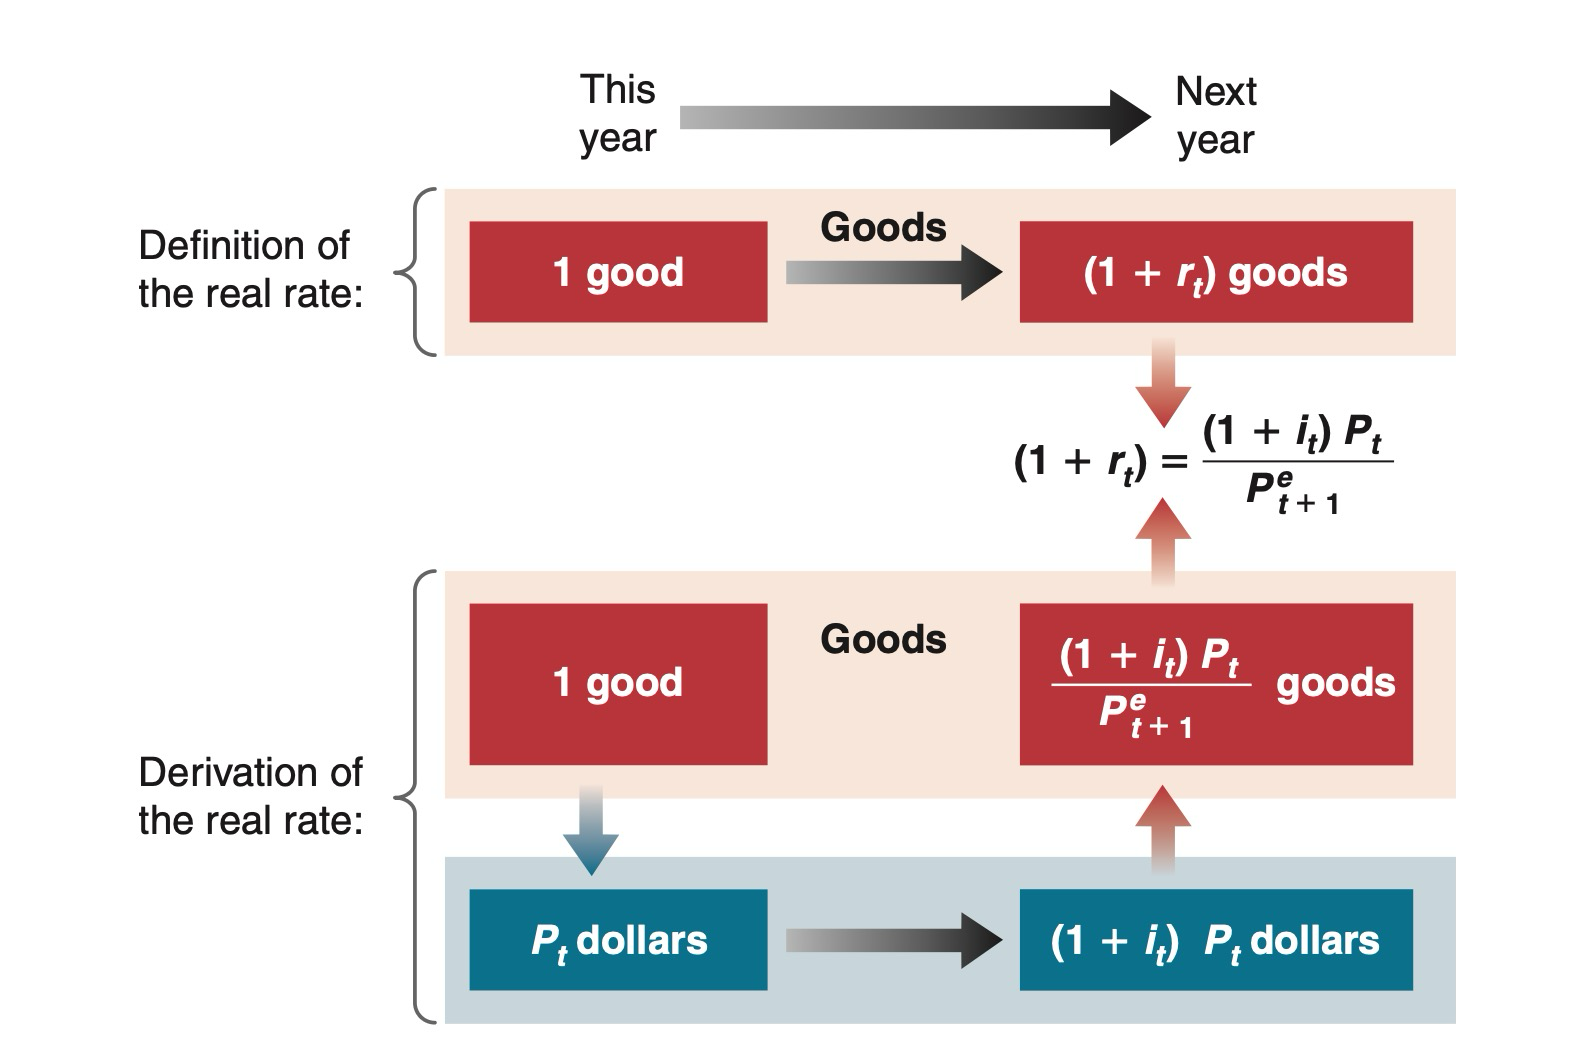
\includegraphics[width=0.5\linewidth]{derivation.png} 
    \caption{Definition and Derivation of the Real Interest Rate} 
    \label{fig:derivation} 
\end{figure}

When we use interest rates, what we truly care about is how many goods can we get in the future. For example, suppose that we just had a barter system, so I borrow/eat a pound of bread from a baker in year $t$. Then, in terms of a real good, I should pay the baker back one pound and a small percentage of a pound of bread. We call this small percentage $r_t$. Thus, after a year, I should give him $1 + r_t$ pounds of bread. By definition, this is the real interest rate.  

Let us now derive the real interest rate  dollars where we are in a system with currency. So instead of just bartering/trading with the bread directly, I have to exchange money to get bread. Let the price of a pound of bread be $P_t$ dollars, so in dimensional analysis, we show it as $\frac{P_t \text{ dollars}}{1 \text{ pound of bread}}$. Then, we would use the nominal interest rate to then get how much I owe in terms of dollars, so I would owe $(1 + i_t)P_t$ dollars. 
But, what we truly care about is how much do we have to return in terms of a pound of bread. 
Thus, we use expected price of a pound of bread next year ($P^e_{t+1}$) and use dimensional analysis again to get:
$$\frac{(1+i_t) P_t \text{ } \cancel{\text{dollars}}}{1} \times \frac{1 \text{ pound of bread}}{P^e_{t+1} \text{ } \cancel{\text{dollars}}} = \frac{(1+i_t)P_t}{P^e_{t+1}} \text{ pounds of bread}$$

We have now shown two ways to represent how we we pay back the interest of borrowing bread. The first is just bartering between bread ($1+r_t$), and the second is going through monetary system ($\frac{(1+i_t)P_t}{P^e_{t+1}}$). Since the two expressions just represent the same transaction, we then have the equation:
$$(1+r_t) = \frac{(1+i_t)P_t}{P^e_{t+1}}$$
We manipulate this equation and use a lot of approximations to eventually get:
$$r_t \approx i_t - \pi^e_{t+1}$$
Thus, the zero lower bound on the nominal interest rate ($i$) implies that the real interest rate ($r$) cannot be lower than expected inflation ($\pi^e$).
\section{Risk and Risk Premia}
In general, people do not like risk. That's why many just invest in government bonds since they can always just print the money when needed. Thus, the expected value of a riskless bond is just $1+i$, where $i$ is the nominal interest rate. However, firms are not the government and can't just print money in demand. As such, they actually have a probability of defaulting (not paying their liabilities). If there is a probability $p$ of the firm defaulting, then the firm has to offer a higher interest rate to make it worth it. Formally, we say that the expected value of a bond with risk must match the expected value of a riskless bond, and firms do this by having a risk premium ($x$). Thus, the following relation must hold:
$$
(1+i) =
\underbrace{(1-p)(1+x+i)}_{\substack{\text{If firm does not default,}\\ \text{loaner receives $1+x+i$ dollars}}}
+
\underbrace{p(0)}_{\substack{\text{If firm defaults,}\\ \text{loaner receives 0 dollars}}}
$$

Isolating for x, we get:
$$x = \frac{(1+i)p}{(1-p)}$$
However, people have a degree of risk aversion. As such, you would usually need an even higher risk premium than what the formula above suggests. For the role of financial intermediaries, I am not explaining that. The book summarizes it best as:
\begin{quote}
``The lower the liquidity of the assets (i.e., the more difficult they are to sell), the
higher the risk of fire sales and the risk that the bank becomes insolvent and goes bank-
rupt. The higher the liquidity of the liabilities (i.e., the easier it is for investors to get their
funds at short notice), the higher the risk of fire sales as well, and the risk that the bank
becomes insolvent and goes bankrupt.''
\end{quote}

\section{Extending IS-LM Model}
From what we have learned, we have two concerns. First, we must distinguish between the nominal interest rate ($i$) and the real interest rate ($r$). Second, we must distinguish the policy rate set by the central bank and the interest rates faced by borrowers.
Both concerns noted actually relate to the IS relation. The first problem was fixed by remembering that borrowers/investors only really care about the real interest rate $r = i - \pi^e$, so we just change the original $I(Y, i)$ into the new $I(Y, i - \pi^e)$. We address the second concern by adding the risk premium $x$ that borrowers/firms face. We thus have:
\begin{align*}
  \text{IS Relation: } Y &= C(Y-T) + I(Y, i - \pi^e + x) + G \\
  \text{LM Relation: } i &= \overline{i}
\end{align*}

Let’s call the rate in the LM equation the nominal policy rate ($i$) because it is determined by monetary policy, and that of the IS equation the real borrowing rate ($r+x$)because it is the rate at which consumers and firms can borrow. We can simplify the equations above by assuming that the central bank just chooses the nominal interest rate to have its target real interest rate. Thus, the central bank chooses the real interest rate directly, and we have:
\begin{align*}
  \text{IS Relation: } Y &= C(Y-T) + I(Y, r + x) + G \\
  \text{LM Relation: } r &= \overline{r}
\end{align*}

I am not going to write anymore about the financial crash of 2008. In my summaries, I will write about the math for the equations since those are usually the most confusing.
\end{document}